\documentclass[10pt,dvips]{article}

\usepackage{../pplmanual}
%%% Commonly Needed packages
\usepackage{graphicx,color,calc}
\usepackage{fancyvrb}
\usepackage{makeidx}
\usepackage{alltt}
\usepackage[linkbordercolor=(0 0 1),citebordercolor=(0 1 0)]{hyperref}
%%\usepackage{xspace} <- creates problems with other hyperlink packages like "html"

%%% Commands for uniform looks of C++, Charm++, and Projections
\newcommand{\CC}{C\hbox{++}}
\newcommand{\emCC}{C\hbox{\em++}}
\newcommand{\charmpp}{\textsc{Charm++}}
\newcommand{\charmc}{\texttt{charmc}}
\newcommand{\projections}{\textsc{Projections}}
\newcommand{\converse}{\textsc{Converse}}
\newcommand{\ampi}{\textsc{AMPI}}
\newcommand{\tempo}{\textsc{TeMPO}}
\newcommand{\irecv}{\textsl{iRecv}}
\newcommand{\sdag}{\textsl{Structured Dagger}}
\newcommand{\jade}{Jade}

%%% Commands to produce margin symbols
\newcommand{\new}{\marginpar{\fbox{\bf$\mathcal{NEW}$}}}
\newcommand{\important}{\marginpar{\fbox{\bf\Huge !}}}
\newcommand{\experimental}{\marginpar{\fbox{\bf\Huge $\beta$}}}

%%% Commands for manual elements
\newcommand{\zap}[1]{ }
\newcommand{\function}[1]{{\noindent{\textsf{#1}}\\}}
\newcommand{\cmd}[1]{{\noindent{\textsf{#1}}\\}}
\newcommand{\args}[1]{\hspace*{2em}{\texttt{#1}}\\}
\newcommand{\prototype}[1]{\vspace{0.2in}\index{#1}}
\newcommand{\param}[1]{{\texttt{#1}}}
\newcommand{\kw}[1]{{\textsf{#1}\index{#1}}}
\newcommand{\uw}[1]{{\textsl{#1}}}
\newcommand{\desc}[1]{\indent{#1}}
\newcommand{\note}[1]{(\textbf{Note:} #1)}
\newcommand{\term}[1]{{\bf #1}\index{#1}}

\makeindex


\title{\Charm Debugger{} Manual}
\version{0.1}
\credits{
By Rashmi Jyothi, Orion Lawlor, Eric Bohm
}
%%Rashmi didn't actually write the manual, but she wrote the debugger and I'm cutting and pasting much of this document from her thesis and the _Debugging in the Context of Charm++_ paper written by Rashmi and Orion.
\begin{document}
\section{Introduction}

The primary goal of the parallel debugger is to provide an integrated
debugging environment which allows the programmer to examine the
changing state of the parallel program during the course of its
execution.

The \charmpp{} debugging system has a number of useful features for
\charmpp{} programmers.  The system includes a Java GUI client program
which runs on the programmer's desktop, and a \charmpp{} parallel
program which acts as a server.  The client and server need not be on
the same machine, and communicate over the network using a secure
protocol described in
 http://charm.cs.uiuc.edu/manuals/html/converse/5\_CONVERSE\_Client\_Server\_In.html 

The system provides the following features: 

\begin{itemize}

\item Provides a means to easily access and view the major programmer
visible entities, including array elements and messages in queues,
across the parallel machine during program execution.  Objects and
messages are extracted using the \charmpp{} PUP framework described in
Section%%~\ref{section:pup}.

\item Provides an interface to set and remove breakpoints on remote
entry points, which capture the major
programmer-visible control flows in a \charmpp{} program. 

\item Provides the ability to freeze and unfreeze the execution of 
selected processors of the parallel program, which allows a 
consistent snapshot by 
preventing things from changing as they are examined.

\item Provides a way to attach a sequential debugger to a specific
subset of processes of the parallel program during execution,
which keeps a manageable number of sequential debugger windows open.

\end{itemize}

The debugging client provides these features via 
extensive support built into the \charmpp{} runtime.

\section{Building the \charmpp{} Debug Tool}

To build the debugger, checkout a fresh copy of charm and then.

\begin{verbatim}
  cd charm/java;
  make;
\end{verbatim}

will create charm/bin/charmdebug for you. 

\section{Preparing the \charmpp Application for Debugging}

No instrumentation is required to use the \charmpp{} debugger.  Being
CCS based, you can use it to set and step through entry point
breakpoints and examine \charmpp{} structures on any \charmpp{}
application.

\subsection{Record Replay}

The \textit{Record Replay} feature is independant of the charmdebug
application.  It is a mechanism used to detect bugs that happen only
once in a while depending on the order in which messages are
processed. The program in consideration is first run in a record mode
which produces a trace. When the program is run in replay mode it uses
a previous trace got from a record run to ensure that messages are
processed in the same order as the recorded run. The idea is to make
use of a message-sequence number and a theorem says that the serial
numbers will be the same if the messages are processed in the same
order. \cite{rashmithesis}

\begin{description}

\item[{\tt -tracemode} {\em recordreplay}]

To enable the required tracing for record and replay, a \charmpp{} 
program is linked with the option ``\textit{-tracemode recordreplay}''
and run with the ``\textit{+record}'' option, which records messages
in order in a file for each processor.  The same execution order can be 
replayed using the ``\textit{+replay}'' runtime option; which can be 
used at the same time as the other debugging tools in \charmpp{}.

\emph{ Note! } If your \charmpp{} is built with {\tt CMK\_OPTIMIZE} on, all tracing will be disabled.  So, use an unoptimized \charmpp{} to do your debugging.

\end{description}

\subsection{GDB}

Although no other intrumentation is required, if you expect a need to
use gdb (or another serial debugger) on one or more of your processes,
compiling your application with the -g flag will maximize its
effectiveness.

\section{Running the Debugger}

\subsection{Charmdebug command line parameters}

\begin{description}

\item[{\tt -pes}] Number of PEs 

\item[{\tt +p}] Number of PEs 

\item[{\tt -host}] hostname of CCS server for application

\item[{\tt -port}] portnumber of CCS server for application

\item[{\tt -display}] X Display

\end{description}

\subsection{Basic usage}

To run an application locally via the debugger on 4 pes with command line options for your pgm (e.g. opt1 opt2 ):

\begin{verbatim}
  charmdebug pgm +p4 4 opt1 opt2
\end{verbatim}

Charmdebug can also be executed without any parameters.  The user can
then choose the application to launch and its command line parameters
from within the \texttt{File} menu as shown in Figure~\ref{menu}.

\begin{figure}[]
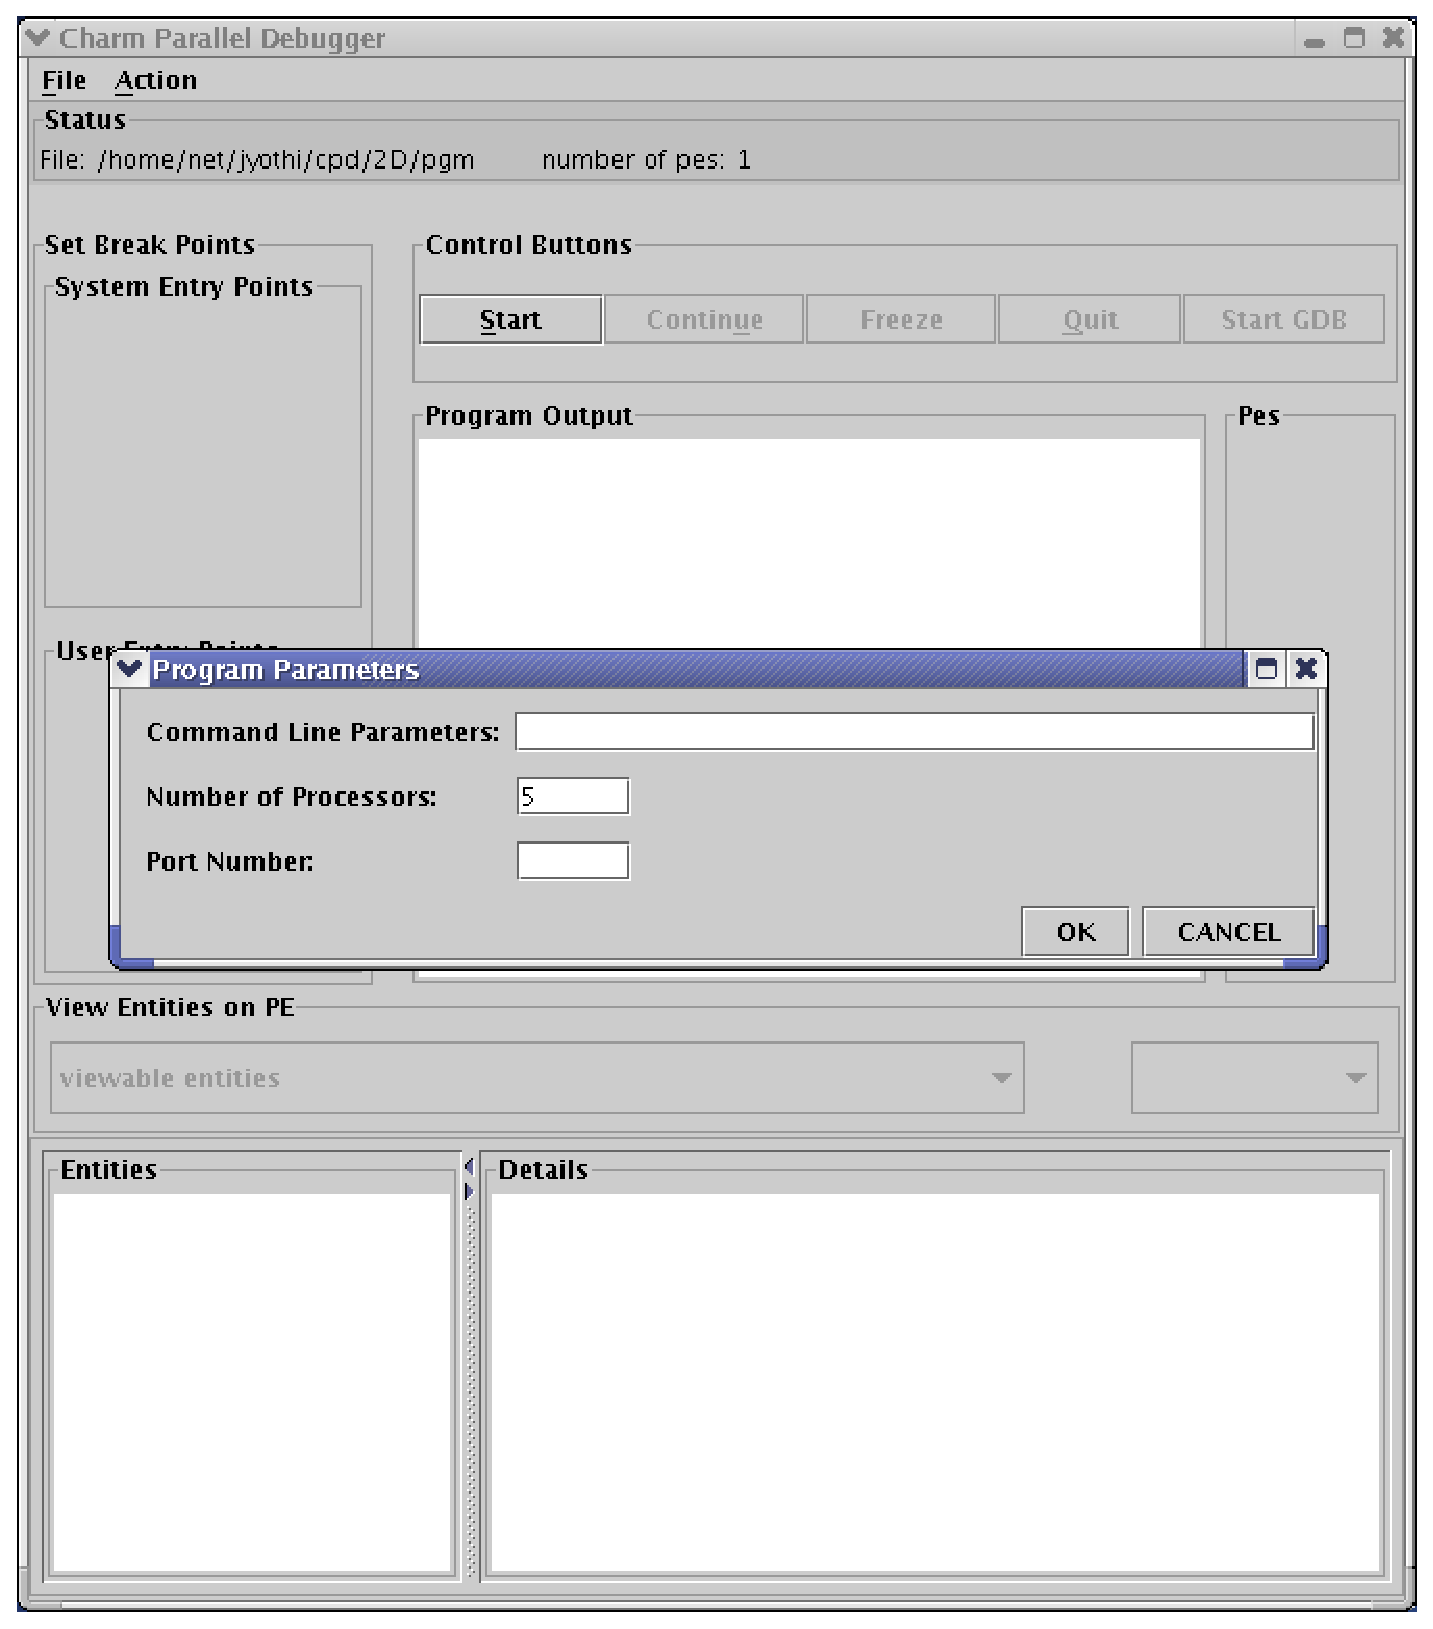
\includegraphics[scale=0.5, height=3in, width=3in]{figs/menu}
\caption{Using the menu to set parameters for the \charmpp{} program}
\label{menu}
\end{figure}




\emph{Note: charmdebug command line launching only works on net-*
builds of \charmpp{} }

To replay a previously recorded session:

\begin{verbatim}
  charmdebug pgm +p4 opt1 opt2  +replay
\end{verbatim}

%%uncomment this when we fix the debugger so it works remotely

%% \subsection{Connecting to a running application}

%% To connect the debugger to a previously launched application.  The
%% application needs to have been launched with the ccs server feature
%% enabled.

%% \begin{verbatim}
%%   charmrun pgm ++server ++server-port 29999
%%   charmdebug pgm -port 29999
%% \end{verbatim}


%% \subsection{Connecting to a remote application}
%% \begin{verbatim}
%%   charmdebug pgm +p4 opt1 opt2   -host remotehost -port 29999
%% \end{verbatim}

%% To have your application freeze upon start so you can initiate flow
%% control via the debugger.
%% \begin{verbatim}
%%   charmdebug pgm +p4 opt1 opt2   -host remotehost -port 29999 +cpd
%% \end{verbatim}

\subsection{Charm Debugging Related Options}

Using the charm debugger to launch your application will set these
to defaults appropriate for most situations.

\begin{description}

\item[{\tt +cpd}] Triggers application freeze at startup for debugger.

\item[{\tt +debugger}] which debuggers to use

\item[{\tt ++debug}] Run each node under gdb in an xterm window, prompting
the user to begin execution.

\item[{\tt ++debug-no-pause}] Run each node under gdb in an xterm window
immediately (i.e. without prompting the user to begin execution).

 \emph{ Note: } If you're using the charm debugger it will probably be
 best to control the sequential (i.e. gdb) debuggers from within its
 GUI interface.
 
\item[{\tt ++display}]          X Display for xterm

\item[{\tt ++server-port}]      Port to listen for CCS requests

\item[{\tt ++server}]           Enable client-server (CCS) mode

\item[{\tt +record}]           Use the recordreplay tracemode to record the exact event/message sequence for later use.  

\item[{\tt +replay}]           Force the use of recorded log of events/messages  to exactly reproduce a previous run.

  The preceding pair of commands {\tt +record +replay} are used to
  produce the ``instant replay'' feature.  This feature is valuable
  for catching errors which only occur sporadically.  Such bugs which
  arise from the nondeterminacy of parallel execution can be
  fiendishly difficult to replicate in a debugging environment.
  Typical usage is to keep running the application with +record until
  the bug occurs.  Then run the application under the debugger with
  the +replay option.

\end{description}

\subsection{Charmdebug limitations}

\subsubsection{Clusters}

Charmdebug is currently limited to local applications due to
implementation peculiarities.  It will be extended to support
connection to remote applications in the near future.  Behavior on a
cluster can be recorded and then replayed in a local run.

\subsubsection{Record Replay}
The \texttt{record replay} feature does not work well with spontaneous
events.  Load balancing is the most common form of spontaneous event
in that it occurs periodically with no other causal event. As per

\begin{figure}[]
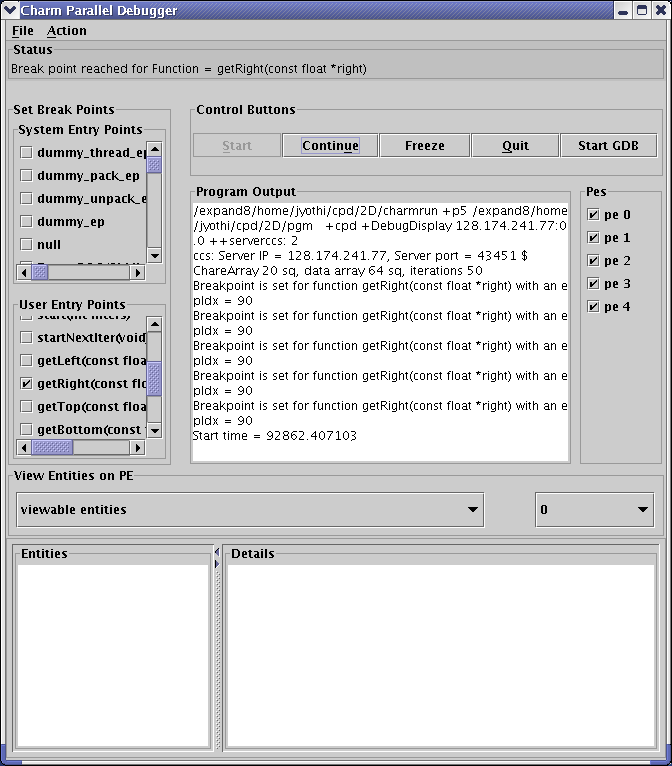
\includegraphics[scale=0.5,height=4in, width=3in]{figs/snapshot3}
\caption{Parallel debugger when a break point is reached}
\label{snapshot3}
\end{figure}

As per Rashmi's thesis: \textit{ There are some unique issues for
replay in the context of Charm because it provides high-level support
for dynamic load balancing, quiescence detection and information
sharing. Many of the load balancing strategies in Charm have a
spontaneous component. The strategy periodically checks the sizes of
the queues on the local processor. A replay load balancing strategy
implements the known load redistribution. The behavior of the old
balancing strategy is therefore not replayed only its effect is. Since
minimal tracing is used by the replay mechanism the amount of
perturbation due to tracing is reduced. The replay mechanism is
proposed as a debugging support to replay asynchronous message arrival
orders.}



\subsection{Using the Debugger}


Once the debugger's GUI loads the programmer triggers the program
execution by clicking the \textit{Start} button.  The program starts
off displaying the user and system entry points as a list of check
boxes, freezing at the onset. The user could choose to set breakpoints
by clicking on the corresponding entry points and kick off execution
by clicking the \textit{Continue} Button. Figure \ref{snapshot3} shows
a snapshot of the debugger when a breakpoint is reached. The program
freezes when a breakpoint is reached.

 
Clicking the \textit{Freeze} button during the execution of the program freezes execution, while
\textit{Continue} button resumes execution. \textit{Quit} button can be used to suspend execution
at any point of time. Entities (for instance, array elements) and their contents on any processor 
can be viewed at any point in time during execution as illustrated in Figure \ref{arrayelement}.

\begin{figure}[]
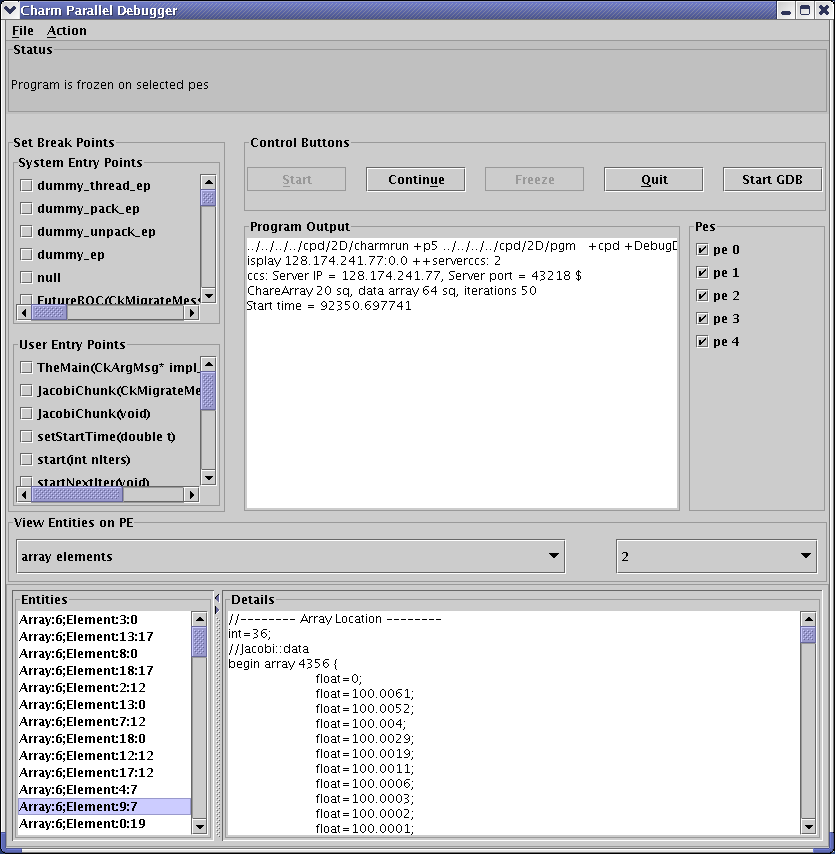
\includegraphics[scale=0.5, height=4in,width=3in]{figs/arrayelement}
\caption{Freezing program execution and viewing the contents of an array element using the Parallel Debugger}
\label{arrayelement}
\end{figure} 

Specific individual processes of the \charmpp{} program can be attached to instances of \textit{gdb} 
as shown in Figure \ref{snapshot4}.  The programmer chooses which PEs to connect \textit{gdb} processes to via the checkboxes on the right side.  


\charmpp{} objects can be examined via  the \textit{View Entities on PE : Display} \ selector.  It allows the user to choose from  \textit{Array Elements, Messages in Queue, Readonly Variables, Readonly Messages, Entry Points, Chare Types, Message Types, Mainchares, and Viewable Lists}.  The right sideselector sets the PE upon whitoThe user may then click on the \textit{Entity} to see the details. 

The programmer can implement the function \texttt{pupCpdData(PUP::er
\&)} for an array element and thereby control the information
displayed by the debugger by choosing the data to be displayed and by
inserting appropriate comments. An example is illustrated in Figure
\ref{instr}.

\begin{figure}[]
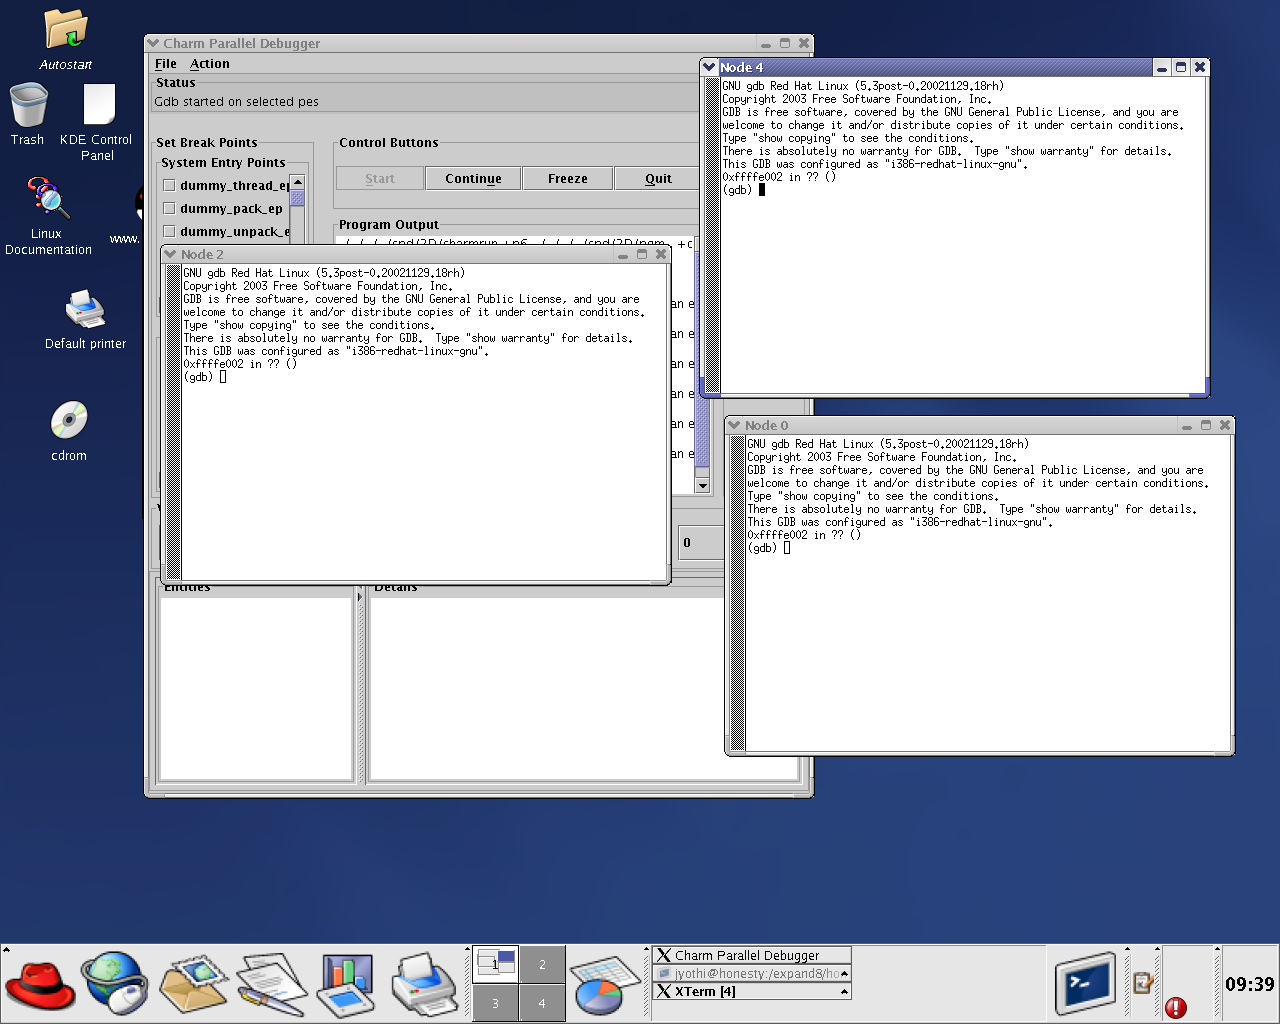
\includegraphics[scale=0.75,height=6in, width=6in]{figs/snapshot4}
\caption{Parallel debugger showing instances of \textit{gdb}
open for the selected processor elements}
\label{snapshot4}
\end{figure}

\begin{verbatim}
// MyArray is a chare array where each array
// element has a member variable data, 
// which is an integer array

void MyArray::pupCpdData(PUP::er &p) {
  p.comment("contents of integer array: data");
  p|data;  }
\end{verbatim}

\section{Debugger Implementation Details}

The following classes in the PUP framework were used in
implementing debugging support in charm.


\begin{itemize}

\item

\texttt{class PUP::er} - This class is the abstract superclass of
all the other classes in the framework. The \texttt{pup} method of
a particular class takes a reference to a \texttt{PUP::er} as
parameter. This class has methods for dealing with all the basic
C++ data types. All these methods are expressed in terms of a
generic pure virtual method. Subclasses only need to provide the
generic method.

\item

\texttt{class PUP::toText} - This is a subclass of the
\texttt{PUP::toTextUtil} class which is a subclass of the
\texttt{PUP::er} class. It copies the data of an object to a C
string, including the terminating NULL.

\item

\texttt{class PUP::sizerText} - This is a subclass of the
\texttt{PUP::toTextUtil} class which is a subclass of the
\texttt{PUP::er} class. It returns the number of characters
including the terminating NULL and is used by the
\texttt{PUP::toText} object to allocate space for building the C
string.

\end{itemize}


The code below shows a simple class declaration
that includes a \texttt{pup} method.


\begin{verbatim}
  class foo {
   private:
    bool isBar;
    int x;
    char y;
    unsigned long z;
    float q[3];
   public:
    void pup(PUP::er &p) {
      p(isBar);
      p(x);p(y);p(z);
      p(q,3);
    }
  };
\end{verbatim}


\subsection{Converse Client-Server Interface}

The Converse Client-Server (CCS) module enables Converse
\cite{InterOpIPPS96} programs to act as parallel servers,
responding to requests from non-Converse programs. The CCS module
is split into two parts - client and server. The server side is
used by a Converse program while the client side is used by
arbitrary non-Converse programs. A CCS client accesses a running
Converse program by talking to a \texttt{server-host} which
receives the CCS requests and relays them to the appropriate
processor. The \texttt{server-host} is \texttt{charmrun}
\cite{charmman} for net-versions and is the first processor for
all other versions.

In the case of the net-version of \charmpp{}, a Converse program
is started as a server by running the \charmpp{} program using the
additional runtime option ``\textit{++server}''. This opens the CCS
server on any TCP port number. The TCP port number can be
specified using the command-line option ``\textit{server-port}''. A
CCS client connects to a CCS server, asks a server PE to execute a
pre-registered handler and receives the response data. The
function \texttt{CcsConnect} takes a pointer to a
\texttt{CcsServer} as an argument and connects to the given CCS
server. The functions \texttt{CcsNumNodes}, \texttt{CcsNumPes},
\texttt{CcsNodeSize} implemented as part of the client interface
in \charmpp{} returns information about the parallel machine. The
function \texttt{CcsSendRequest} takes a handler ID and the
destination processor number as arguments and asks the server to
execute the particular handler on the specified processor.
\texttt{CcsRecvResponse} receives a response to the previous
request in-place. A timeout is also specified which gives the
number of seconds to wait till the function returns a 0, otherwise
the number of bytes received is returned.

Once a request arrives on a CCS server socket, the CCS server
runtime looks up the appropriate registered handler and calls it.
If no handler is found the runtime prints a diagnostic and ignores
the message. If the CCS module is disabled in the core, all CCS
routines become macros returning 0. The function
\texttt{CcsRegisterHandler} is used to register handlers in the
CCS server. A handler ID string and a function pointer are passed
as parameters. A table of strings corresponding to appropriate
function pointers is created. Various built-in functions are
provided which can be called from within a CCS handler. The
debugger behaves as a CCS client invoking appropriate handlers
which makes use of some of these functions. Some of the built-in
functions are as follows.

\begin{itemize}

\item

\texttt{CcsSendReply} - This function sends the data provided as
an argument back to the client as a reply. This function can only
be called from a CCS handler invoked remotely.

\item

\texttt{CcsDelayReply} - This call is made to allow a CCS reply to
be delayed until after the handler has completed.


\end{itemize}

The CCS runtime system provides several built-in CCS handlers,
which are available to any Converse program. All \charmpp{}
programs are essentially Converse programs. \texttt{ccs\_getinfo}
takes an empty message and responds with information about the
parallel job. Similarly the handler \texttt{ccs\_killport} allows
a client to be notified when a parallel run exits.

\end{document}
